\chapter{Elevating Aermax – First Sprint Enhancements and Integrations}

\section{Introduction}
In this chapter, we cover the first sprint of the Aermax project, focusing on team collaboration and meetings, as well as the key enhancements and features we implemented to improve the platform.

\section{Team Collaboration and Meetings}

\subsection{Daily Standups}
\textbf{Purpose:} Share daily progress, plan the day, and address blockers. \\
\textbf{Structure:} Each team member provides a brief update on:
\begin{itemize}
    \item What they did yesterday.
    \item What they plan to do today.
    \item Any blockers they are facing.
\end{itemize}

\subsection{Retrospectives}
\textbf{Purpose:} Discuss what went well, what didn’t, and identify areas for improvement. \\
\textbf{Outcome:} Action items to enhance future sprints.

\subsection{Client Meetings}
\textbf{Initial Requirements Gathering:} Detailed discussions to understand client needs. \\
\textbf{Ongoing Feedback Sessions:} Regular updates to demonstrate progress and gather feedback.
\begin{figure}[H]
    \centering
    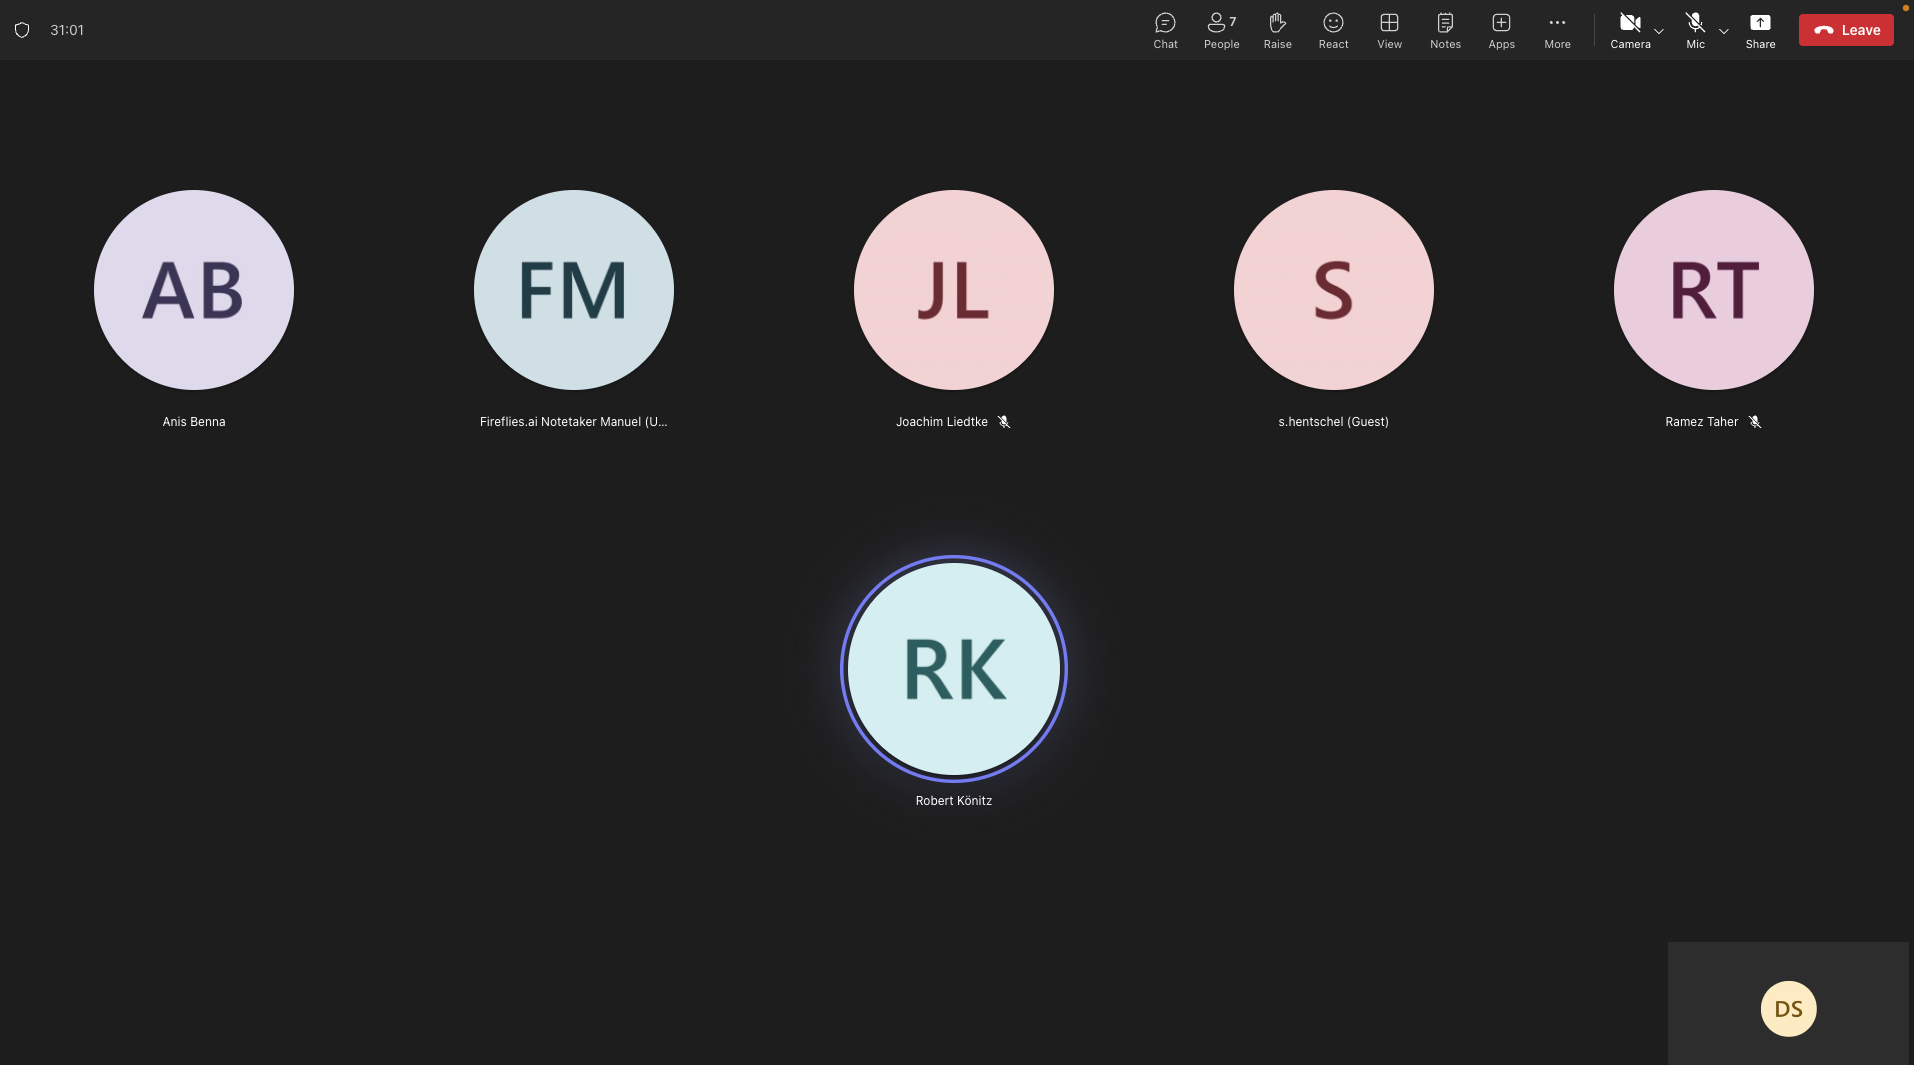
\includegraphics[width=0.9\textwidth]{src/assets/chapters/JF MEETING.png}
    \caption{Screenshot of Video Call with Client}
    \label{fig:client_meeting}
\end{figure}
\begin{figure}[H]
    \centering
    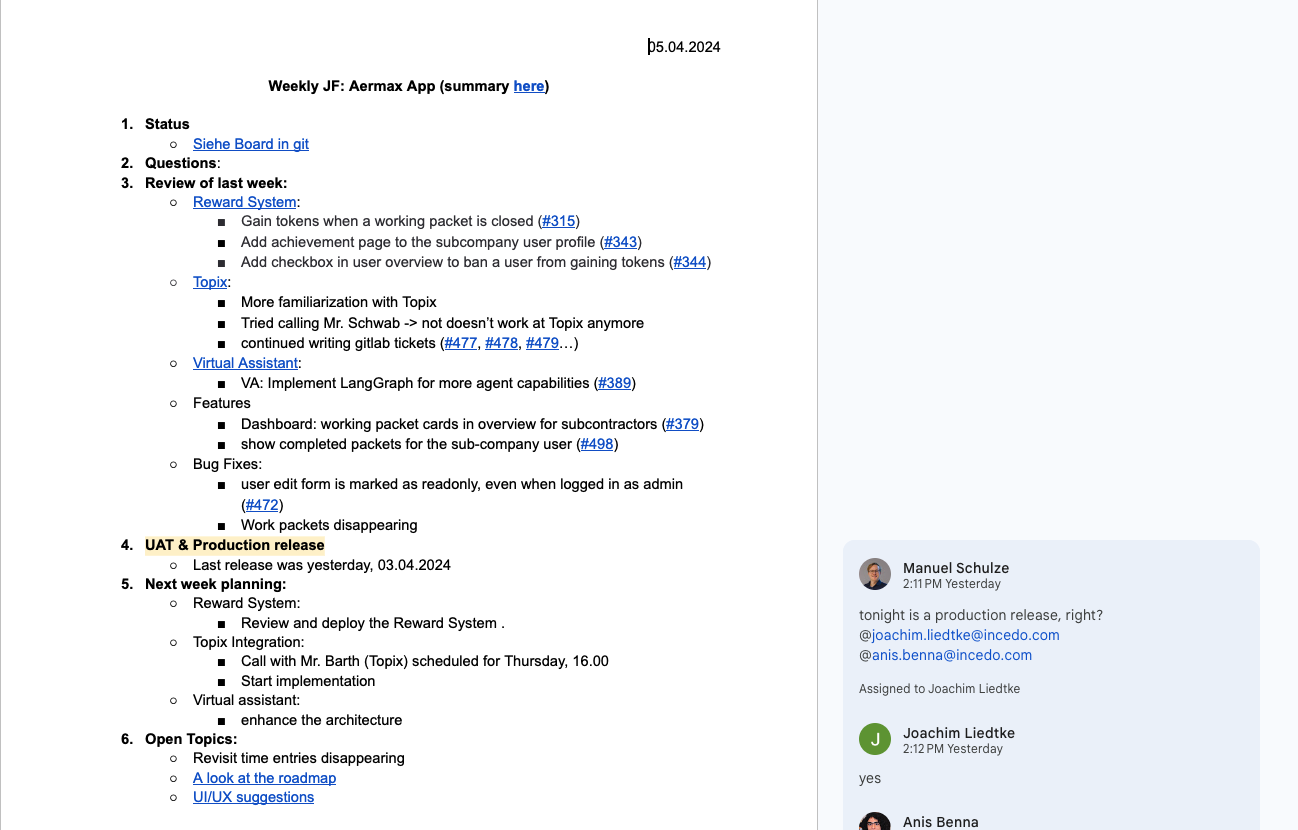
\includegraphics[width=0.9\textwidth]{src/assets/chapters/JF.png}
    \caption{ Weekly JF Meeting Summary Log for the Aermax App Project}
    \label{fig:Weekly_JF}
\end{figure}

\subsection{Ticket Management and Workflow}
\textbf{Tool:} Use of GitLab for managing tasks. \\
\textbf{Process:} Tickets are created, assigned, and tracked through stages like "To Do," "In Progress," "In Review," and "Done."
\begin{figure}[H]
    \centering
    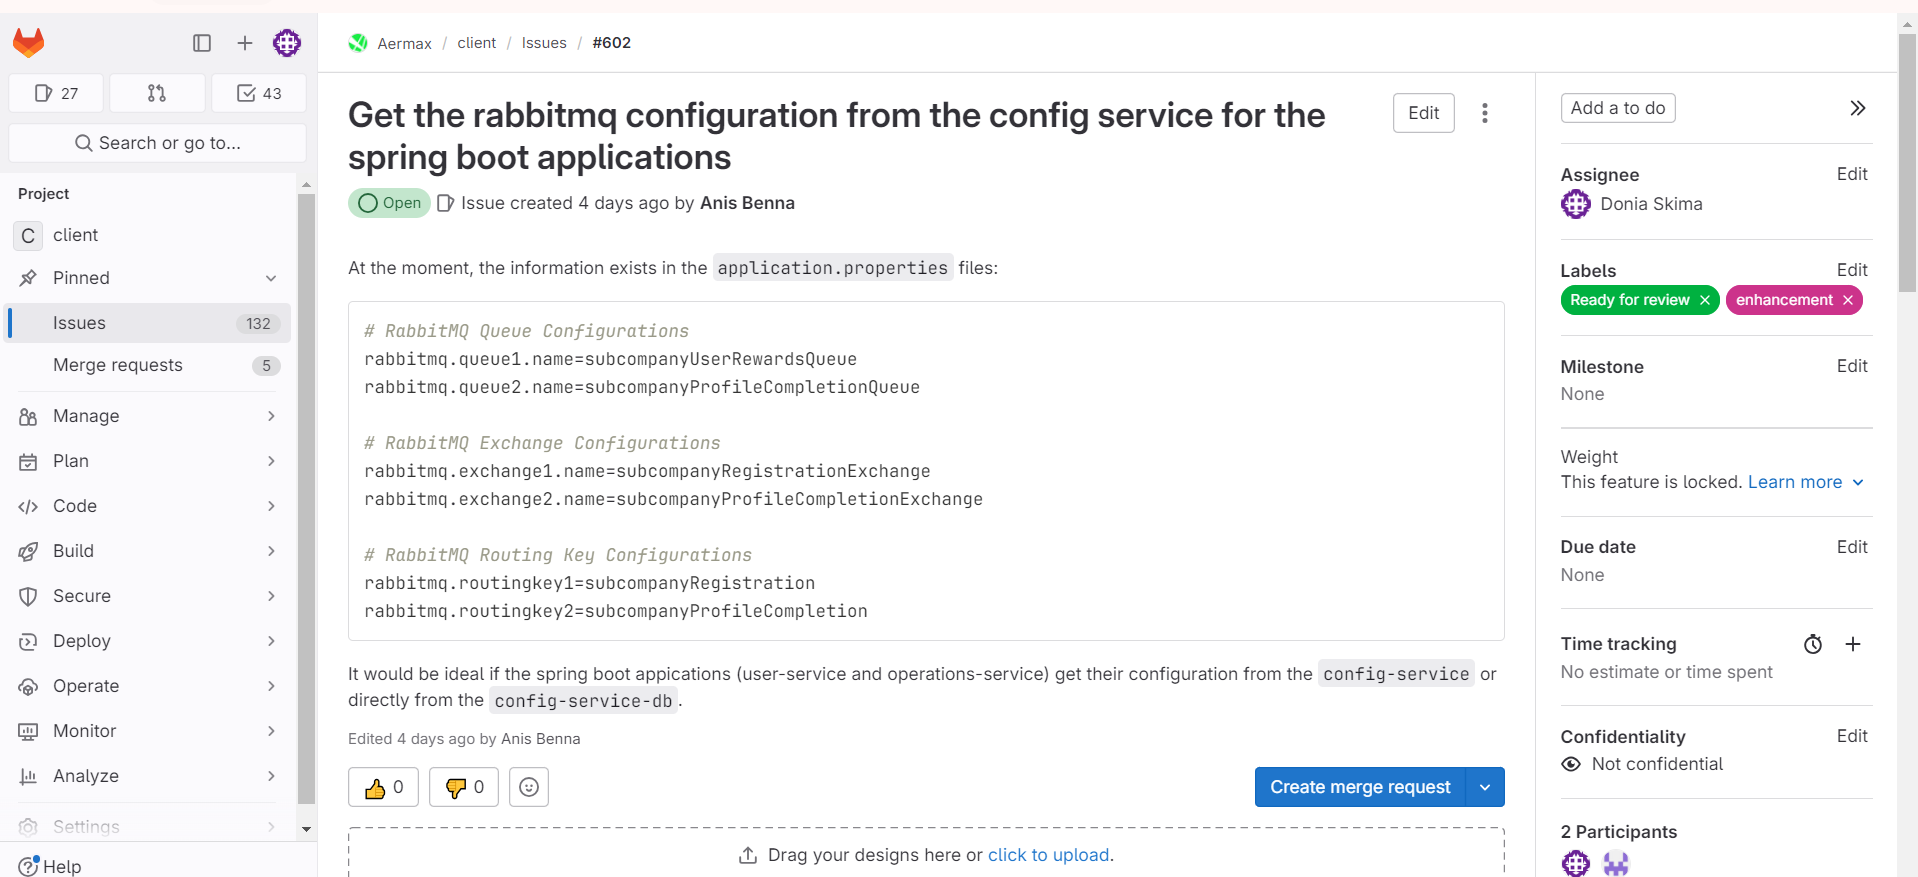
\includegraphics[width=0.9\textwidth]{src/assets/chapters/ticket.PNG}
    \caption{Example of Ticket in GitLab}
    \label{fig:ticket_management}
\end{figure}

\subsection{Communication Tools}
\textbf{Microsoft Teams:} For instant messaging. \\
\textbf{Microsoft Teams/Google Meet:} For video conferencing. \\
\textbf{Google Docs:} For documentation and collaborative editing.
\begin{figure}[H]
    \centering
    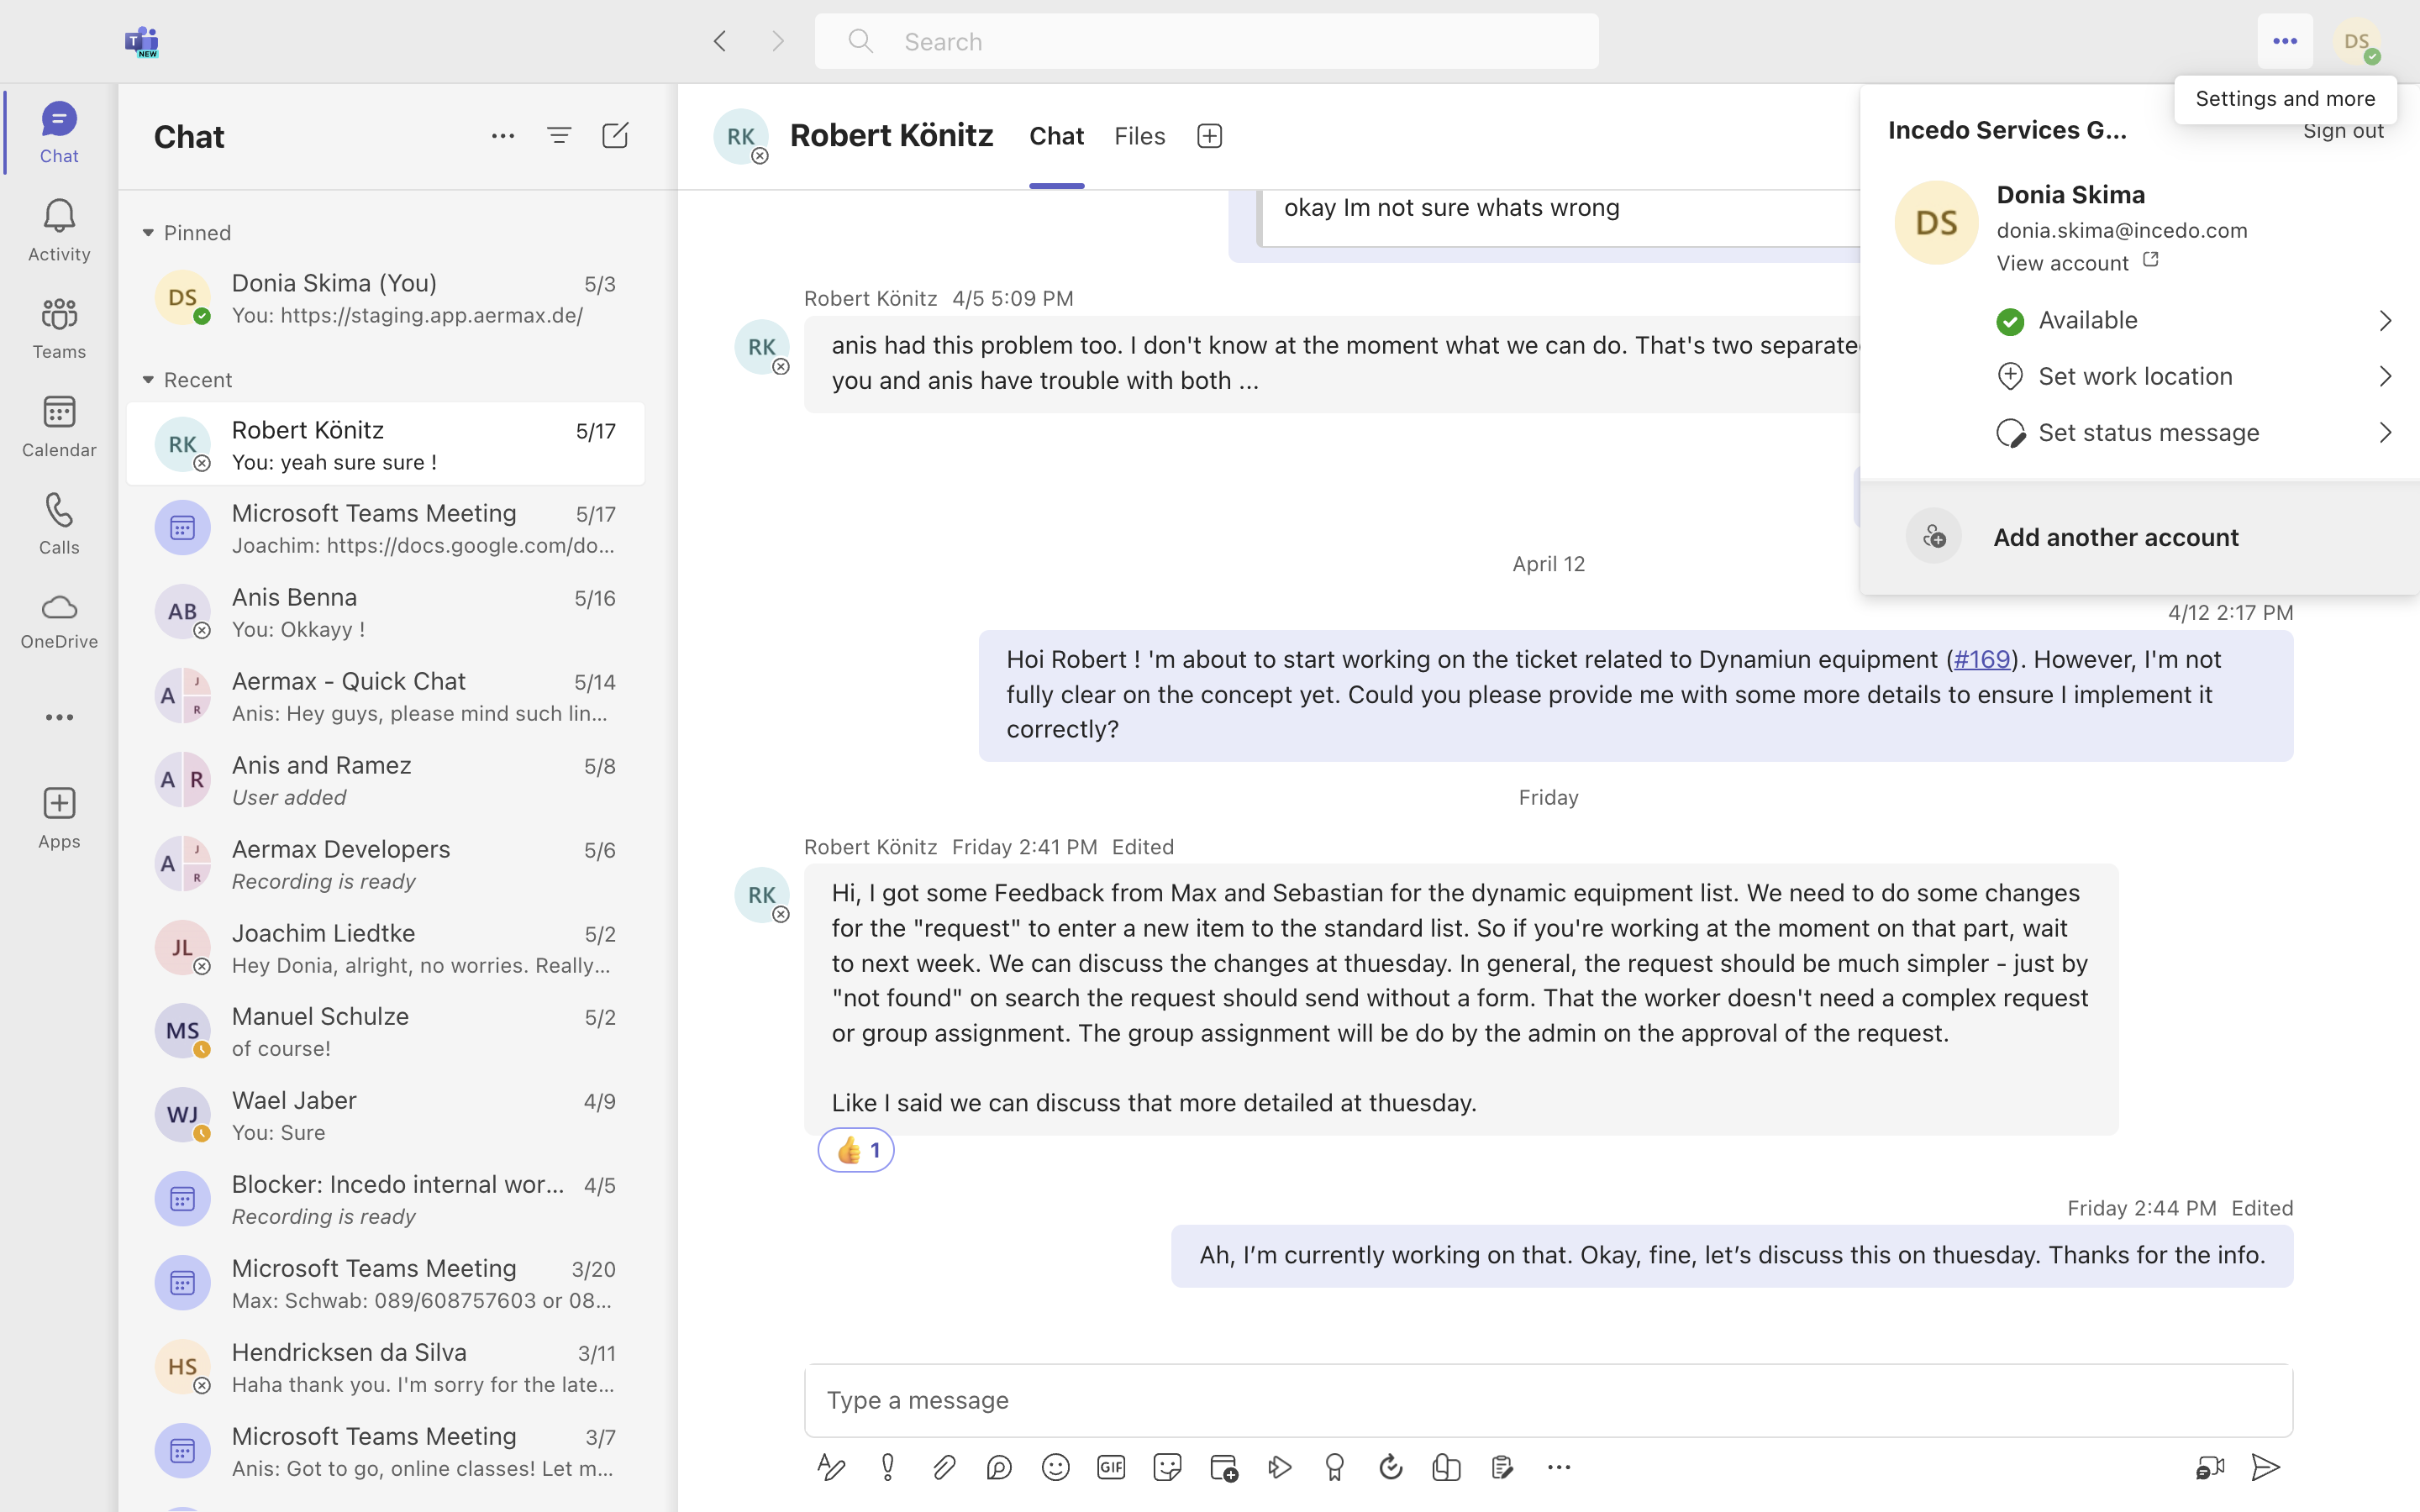
\includegraphics[width=0.9\textwidth]{src/assets/chapters/MicrosoftTeams.png}
    \caption{Screenshot of Microsoft Teams in Use}
    \label{fig:communication_tools}
\end{figure}

\section{Major Features and Enhancements}
